\chapter{The Standard Model of Particle Physics}
\label{chapter:SM}

\begin{table}[!htb]
    \begin{center}
        \begin{tabularx}{0.8\textwidth}{m{1em} c c c c c c c }
        \toprule
        \hline
& Field & Members & Spin & \Uone$_{Y}$) & \SUtwo$_{L}$ & \SUthree$_{C}$ \\
        \hline

        %\rotatebox{90}{\hspace{-0.1cm}\textbf{Fermionic Field} }
            \rotatebox{90}{\hspace{-0.1cm}\textbf{Leptons} }
             &   \makecell{\fieldLi \\ \fieldEri} % FIELD
             &   \makecell{ (\fieldEl, \fieldNuEl), (\fieldMul, \fieldNuMul), (\fieldTaul, \fieldNuTaul) \\ \fieldEr, \fieldMur, \fieldTaur}% CONTENT
             &   \makecell{ $1/2$ \\ $1/2$ }% SPIN
             &   \makecell{ $-1$ \\ $-2$ }% U(1)
             &   \makecell{ $\mathbf{2}$ \\ $\mathbf{1}$ }% SU(2)
             &   \makecell{ $\mathbf{1}$ \\ $\mathbf{1}$ } \\ % SU(3)
            \midrule
            \rotatebox{90}{\hspace{-0.1cm}\textbf{Quarks} } 
             &   \makecell{\fieldQi \\ \fieldUri \\ \fieldDri} % FIELD
             &   \makecell{ (\fieldUl, \fieldDl), (\fieldCl, \fieldSl), (\fieldTl, \fieldBl) \\ \fieldUr \\ \fieldDr}% CONTENT
             &   \makecell{ $1/2$ \\ $1/2$ \\ $1/2$} % SPIN
             &   \makecell{ $1/3$ \\ $4/3$ \\ $-2/3$}% U(1)
             &   \makecell{ $\mathbf{2}$ \\ $\mathbf{1}$ \\ $\mathbf{1}$}% SU(2)
             &   \makecell{ $\mathbf{3}$ \\ $\mathbf{3}$ \\ $\mathbf{3}$}\\ % SU(3)

        \cdashline{1-7}

        %\rotatebox{90}{\hspace{-0.1cm}\textbf{Bosonic Field} }
            \rotatebox{90}{\textbf{\stackanchor{Gauge}{Fields}} }
             &   \makecell{\fieldB \\ \fieldW \\ \fieldG } % FIELD
             &   \makecell{ \fieldB \\ (\fieldWone, \fieldWtwo, \fieldWthree) \\ \fieldG$_a$, $a\in[1,..,8]$ }% CONTENT
             &   \makecell{ $1$ \\ $1$ \\ $1$} % SPIN
             &   \makecell{ $0$ \\ $0$ \\ $0$}% U(1)
             &   \makecell{ $\mathbf{1}$ \\ $\mathbf{3}$ \\ $\mathbf{1}$}% SU(2)
             &   \makecell{ $\mathbf{1}$ \\ $\mathbf{1}$ \\ $\mathbf{8}$}\\ % SU(3)
            \midrule
            \rotatebox{90}{\textbf{\stackanchor{Higgs}{Field}}} 
             &   \makecell{\fieldPhi } % FIELD
             &   \makecell{ (\fieldPhip, \fieldPhizero) }% CONTENT
             &   \makecell{ $0$  } % SPIN
             &   \makecell{ $1$  }% U(1)
             &   \makecell{ $\mathbf{2}$ }% SU(2)
             &   \makecell{ $\mathbf{1}$ }\\ % SU(3)
        \hline
        \bottomrule
        \end{tabularx}
    \end{center}

    \caption{
        The particle fields of the SM\cite{Antrim:2699575}.
    \label{table:sm1}
    }

\end{table}

\FloatBarrier


\begin{table}[!htb]
    \caption{
        The table shows the particle fields of the SM after SSB. Coupling and mass parameters are provided. 
    }
        %The particle content of the SM after the process of
        %electroweak symmetry breaking.
        %Shown for each particle species are the associated electric charge, $Q$,
        %coupling, and mass (approximate).
        %The $y_i$ are the Yukawa coupling (Equation~\ref{eq:higgs_fermion_coupling}),
        %$\alpha_{\text{EM}}$ is the QED coupling constant (`fine structure constant'),
        %$\mathcal{V}$ indicates the parameters of the CKM matrix, and
        %$\alpha_s$ is the QCD coupling constant.
        %The quantities $\lambda$ and $\mu$ are the Higgs self-coupling parameter
        %and mass terms, respectively, appearing in Higgs potential terms (Equation~\ref{eq:higgs_potential}).
    \begin{center}
        \begin{tabularx}{1\textwidth}{m{1em} c c c c }
        \toprule
        \hline
        & Physical Field & Q & Coupling & Mass [GeV] \\
        \hline
        \rotatebox{90}{\hspace{-0.1cm}\textbf{Quarks} } 
            & \makecell{ \quarkU, \quarkC, \quarkT \\ \quarkD, \quarkS, \quarkB} % FIELD
            & \makecell{ $2/3$ \\ $-1/3$ }% Q
            %& \makecell{ $\mathbf{3}$ \\ $\mathbf{3}$ } % SU(3)
            & \makecell{ ($y_i=$) $1\times10^{-5}$, $7\times10^{-3}$, $1$ \\ ($y_i=$) $3\times10^{-5}$, $5\times10^{-4}$, $0.02$ } % Coupling
            & \makecell{ $2\times10^{-3}$, $1.27$, $173$ \\ $4\times10^{-4}$, $0.10$, $4.18$ }\\% Mass
        \rotatebox{90}{\hspace{-0.1cm}\textbf{Leptons} } 
            & \makecell{ \leptonE, \leptonMu, \leptonTau \\ \neutrinoE, \neutrinoMu, \neutrinoTau } % FIELD
            & \makecell{ $-1$ \\ $0$ }% Q
            %& \makecell{ $\mathbf{1}$ \\ $\mathbf{1}$ } % SU(3)
            & \makecell{ ($y_i=$) $3\times10^{-7}$, $6\times10^{-4}$, $0.01$ \\ -- } % Coupling
            & \makecell{ $5\times10^{-4}$, $0.106$, $1.777$ \\ --}\\% Mass
        \midrule
        \rotatebox{90}{\textbf{Bosons} } 
            & \makecell{ \fieldPhoton \\ \fieldZ \\ (\fieldWp, \fieldWm) \\ \fieldG } % FIELD
            & \makecell{ $0$ \\ $0$ \\ $(+1,-1)$ \\ $0$ }% Q
            %& \makecell{ $\mathbf{1}$ \\ $\mathbf{1}$ \\ $\mathbf{1}$ \\ $\mathbf{8}$ } % SU(3)
            & \makecell{ $\alpha_{\text{EM}} \simeq 1/137$ \\ $\sin \theta_{W} \simeq 0.5$ \\ $\mathcal{V}_{\text{CKM}}$ \\ $\alpha_s \simeq 0.1$ } % Coupling
            & \makecell{ $0$ \\ $91.2$ \\ $80.4$ \\  $0$}\\% Mass
        \midrule
        \rotatebox{90}{\textbf{Higgs} } 
            & \makecell{ \fieldH } % FIELD
            & \makecell{ $0$ }% Q
            %& \makecell{ $\mathbf{1}$ } % SU(3)
            & \makecell{ $\lambda$, $\mu$ } % Coupling
            & \makecell{ $125.09$ }\\% Mass
        \hline
        \bottomrule
        \end{tabularx}
    \end{center}
    \label{tab:sm_content_EWSB}
\end{table}
    
	
\epigraph{\textit{Ex pede Herculem. \newline(From the feet, Hercules.)}}{--Herodotus, Book IV, Section LXXXII. Plutarch}

The Standard Model of Particle Physics (SM) is the epitome of human understanding of physical elementary building blocks to-date. From the SM, the properties and interactions of seventeen fundamnetal particles and their interactions are laid out. It provides the foundational understanding to matter and their interactions in the quantum scale.

This chapter provides an overview of the SM: In section~\ref{sec:SM} a theoretical description of the SM is given. The mechanism to the theory is discussed. The Gauge fields and their particles are listed. As a complete picture of the SM relies on experimental measurement on its paramters, the measureed values of the eighteen parameters are also catelogued in this section. Despite the many advances made by the SM, there remains many open
questions left to be solved. Some of them are motivators to studies done in this thesis. In section~\ref{sec:UnresolvedSM}, a summarized list of resolved problems to the SM is presented.

\section{Standard Model: Theoretical Description}
\label{sec:SM}

Mathematically, the SM is a gauge theory under the 
Quantum Field Theory (QFT) framework. Particles are represented different quantized fields operators. The particle interactions are determined by the SM Lagrangian which takes the form as shown in the eq~\ref{eq:SMLagrangian}. Through the SM Lagrangian, all physics laws concerning the particle interaction modes, their interaction cross sections and their motion through scattering can be derived.

\subsection{Symmetry}
Symmetry is the corner of many laws in physics. Mathematically, it's the invariance of quantities through transformation, and is shown by the Noether's Theorem to be related to conservation laws in physics:
    \begin{itemize}
        \item Spatial Translational Symmetry $\rightarrow$ Translational Momentum Conservation
        \item Time Symmetry $\rightarrow$ Energy Conservation
        \item Rotational Symmetry $\rightarrow$ Angular Momentum Conservation
    \end{itemize}

    Symmetry and its transformation can be summarized by the mathematical language of group theory. In group theory, continuous transformation is described by the Lie group and the discrete transformation is represented by a finite group. 

    There are two kinds of symmetries in the SM, the external symmetries and internal symmetries. External symmetries are symmteries related to space-time transformation of the particle; Internal particle symmetries that are related to other particle properties other than space-time. 

\subsubsection{External Symmetries} 
The external symmetries are transformations on the space-time coordinates, The SM external symmetries can be summarized by the following three groups, known collectively as the \textit{Poincar\'{e} group}. Each of the terms conserves a physics quantity. 
    
     \begin{equation}
     \textbf{\textit{P}} \times \textbf{\textit{J}} \times \textbf{\textit{K}}
     \end{equation}
     
    \begin{itemize}
        \item \textbf{\textit{P}}: Spatial Translational Symmetry

            Abelian Lie group translation on space-time $\rightarrow$ conserves momentum 
        \item \textbf{\textit{J}}: Rotational Symmetry

            Non-Abelian Lie group of three-dimensional rotation $\rightarrow$ conserves Angular Momentum 
        \item \textbf{\textit{K}}: Boost Symmetry 

            Abelian Lie group of four dimensions $\rightarrow$ conserves \textit{Invariant Interval} in Special relativity.
    \end{itemize}


    The \textit{Invariant Interval} quantity is defined as:

    \begin{equation}
        \Delta s^2 \overset{\mathrm{def}}{=} c^{2}\Delta t^{2} - (\Delta x^{2}+\Delta y^{2} + \Delta z^{2})
        \label{eq:InvariantInterval}
    \end{equation}

    In special relativity, when the space-time measurement of an event is transformed through different frames of references, the \textit{Invariant Interval} remains unchanged. In the equation above, $\Delta s^{2}$ is the \textit{Invariant Interval}, $\Delta t^{2}$ is the difference in time measurements between the two frame of reference, whereas $\Delta x$, $\Delta y$ and $\Delta z$ are the differece in position in between the different frame of references.

\subsubsection{Internal Symmetry}
The SM internal symmetries describe transformation in physical properties of the particles other than space-time. Particle gauge field interaction can be described as "transformations" from one field to another under internal symmetry. The different physical invariant quantities that are conserved under these particle transformations/interactions are called "charges". From these internal symmetries, Charge, Parity and time reversal symmetry (CPT) is observed. 

The internal symmetries is given as:

    \begin{equation}
        \SUthree_{C} \times  \SUtwo_{L} \times \Uone_{Y}
    \end{equation}


    The following symmetries governs the particle interactions under the strong and electro-weak forces. 
    
    The $\SUthree_{C}$ symmetry describes strong force interaction, it only affects the quark gauge field with color charges. 
    
    %The local $SUthree_{C}$ symmetry governs the strong force and only has an effect on particles with a color charge (either red, green, or blue). These particles in the Standard Model include quarks of field $\mathcal{Q}_{i}$. It consist of the left handed doublets of  ($u_{L}$, $d_{L}$), ($c_{L}$, $s_{L}$), ($t_{L}$, $b_{L}$) and right-handed singlets of $u_{R,i}$ and $d_{R}$. The strong force is mediated by the eight gluon fields $\mathcal{G}$.

    The $\SUtwo_{L} x \Uone_{Y}$ transformation describes the weak  and weak hypercharge transformation and is effective on particles gauge field with the weak charge and the weak-hypercharge respectively
    
    The combined effect of the weak field $\SUtwo_{L}$ and the weak hyper-charge field $\Uone_{Y}$ gives the familiar electro-magnetic weak force after spontaneous symmetry breaking. This affects both the quark field and leptonic fields transformations, The detailed mechanism of spontaneous symmetry breaking is given in section~\ref{sec:SSB}.


    A detailed list of the gauge fields and their charges along with their mathematical group and generator under effect can be found in table~\ref{table:sm}.

\subsection{The Lagrangian}

Observing the symmetries given in the above section, the Lagrangian of the SM is written as the following:

\begin{equation}
    \mathcal{L}_{SM}= - \frac{1}{4} \sum\limits_{gauge} F^{i}_{\mu \nv}F^{i\mu\nv} - \sum\limits_{f} \overline{f} \gamma^{\mu} D_{\mu} f +(D_{\mu}\phi)^{\dagger}(D^{\mu}\phi) - \mu^{2}\phi^{\dagger}\phi - \lambda(\phi^{\dagger}\phi)^{2}
    \label{eq:SMLagrangian}
\end{equation}


%The first term is a summation of the gauge fields, the short from of F, where $F^{a}_{\mu\nv}=\patial_{\mu}A_{\nv}^{a}-\partial_{\nv}A_{\mu}^{a}+g f^{abc}A^{b}_{\mu}A^{c}_{\nv}$. $A_{\mu}$ represents a gauge field, g is the gauge coupling parameter, and $f^{abc}$ is the structure constants of the gauge group. 
%
%The second term describes the kinetic energy of the particle fields, the gauge covariant derivative $D_{\mu}$ is a short form, where $D_{\mu}=\partial_{\mu}-i g_{1} \frac{Y}{2}B_{\mu} - i g_{2}\frac{\Tau ^{i}}{2}W_{\mu}^{i} - ig_{3}\frac{\lambda^{a}}{2}G^{a}_{\mu}$. Here, $g_{1}$, $g_{2}$ and $g_{3}$ is the gauge coupling constants. The $\Tau ^{i}$ and $\lambda^{a}$ terms are the respective generators of the $\SUtwo_{L}$ and $\SUthree_{C}$ gauge groups. 
%
%The last terms concerns the Higgs potential. They are discussed in detail in section ~\ref{sec:SSB}.
%

%\subsection{Spontaneous Symmetry Breaking}
%\label{sec:SSB}
%The Standard Model theory in the form as presented in the last section does not give mass to the particles. This inconsistent with observations in experiment.  
%It can be shown that adding ad-hoc mass terms for these particle fields breaks the internal symmetries and are not permitted by the theory. This is solved by the addition of a spin 0 Higgs field. SM particles gain mass through the spontaneous symmetry breaking (SSB) of the field. In the following, a condensed derivation of the SSB is described\cite{peskin2018introduction}.
%
%The Higgs potential is as follows:
%
%\begin{equation}
%    V{\phi} = \mu^{2}\phi^{2} - \lambda \phi^{4}
%\end{equation}
%
%When \mu^{2} takes a negative value, the potential takes on a symmetric shape where the minimum value is not found at 0, but rather at \nv. At this minimum point of the potential, the vacuum expectation value is:
%
%\begin{equation}
%    \phi_{0} = \frac{1}{\sqrt{2}}
%    \begin{pmatrix}
%        0\\
%        \nu
%    \end{pmatrix}
%\end{equation}
%
%In this value, while the overall potential is still symmetric, the particle is no longer at a symmetric equilibrium. The symmetry is spontaneously broken. 
%
%It can be shown that mass can be obtained when a gauge transformation is performed on the vacuum expectation value:
%
%\begin{equation}
%    \phi_{0} = \frac{1}{\sqrt{2}}
%    \begin{pmatrix}
%        0\\
%        \nu+h(x)
%    \end{pmatrix}
%\end{equation}
%
%It leads to the $D_{\mu} \phi$ in the third to last term in the Lagrangian ~\ref{eq:SMLagrangian} to take the following form:
%
%\begin{equation}
%    D_{\mu}\ = (\partial_{\mu}- ig A_{\mu}^{a}\Tau^{a} - i\frac{1}{2}g' B_{\mu}) \phi
%\end{equation}
%
%Plugging this back into the Lagrangian in ~\ref{eq:SMLagrangian}, the change in the Lagrangian will become:
%
%\begin{equation}
%    \Delta \mathcal{L} = \frac{1}{2} \frac{\nv^{2}}{4}[g^{2}(A^{1}_{\mu})^2 + g^{2}(A_{\mu}^{2})^{2} + (-g A_{mu}^{3}+ g'B_{\mu})^2]
%\end{equation}
%
%With the following substitutions:
%
%\begin{equation}
%    W^{\pm}_{\mu} = \frac{1}{\sqrt{2}}(A_{\mu}^{1} \mp iA^{2}_{\mu}) 
%\end{equation}
%
%\begin{equation}
%    Z^{0}_{\mu}=\frac{1}{\sqrt{g^{2}+g'^{2}}}(g'A_{\mu}^{3} + gB_{\mu})
%\end{equation}
%
%\begin{equation}
%    A_{\mu} = \frac{1}{\sqrt{g^{2}+g'^{2}}}(g'A^{3}_{\mu} + g B_{\mu})
%\end{equation}
%
%It can be shown that the mass of the $W^{\pm}$ and $Z_{0}$ boson are:
%
%\begin{equation}
%    m_{W} = g \frac{\nv}{2}
%\end{equation}
%
%\begin{equation}
%    m_{Z} = \sqrt{g^{2}+ g'^{2}\frac{\nv}{2}}
%\end{equation}
%
%The vector fields remains massless:
%
%\begin{equation}
%    m_{A}=0
%\end{equation}
%
%This mass gainning process follows from the Goldstone's Theorem. It states that for each broken continous symmetry, a massless scalar boson will appear. After SSB, the $W^{\pm}$ and Z field acquire mass by 'eating' the degree of freedom from the Goldstone boson. These bosons thereby acquired mass. 
%
%As a consequence, it can be shown that the familiar electric charge as a is the combination the weak and hyperweak coupling:
%
%\begin{equation}
%    e= \frac{g g'}{\sqrt{g^{2}+g'^{2}}}
%\end{equation}
%
%The electric charge quantum number can be written as:
%\begin{equation}
%    Q=T^{3}+Y
%\end{equation}
%
%
\begin{table}[!htb]
    \caption{
        The table shows the particle fields of the SM after SSB. Coupling and mass parameters are provided. 
    }
        %The particle content of the SM after the process of
        %electroweak symmetry breaking.
        %Shown for each particle species are the associated electric charge, $Q$,
        %coupling, and mass (approximate).
        %The $y_i$ are the Yukawa coupling (Equation~\ref{eq:higgs_fermion_coupling}),
        %$\alpha_{\text{EM}}$ is the QED coupling constant (`fine structure constant'),
        %$\mathcal{V}$ indicates the parameters of the CKM matrix, and
        %$\alpha_s$ is the QCD coupling constant.
        %The quantities $\lambda$ and $\mu$ are the Higgs self-coupling parameter
        %and mass terms, respectively, appearing in Higgs potential terms (Equation~\ref{eq:higgs_potential}).
    \begin{center}
        \begin{tabularx}{1\textwidth}{m{1em} c c c c }
        \toprule
        \hline
        & Physical Field & Q & Coupling & Mass [GeV] \\
        \hline
        \rotatebox{90}{\hspace{-0.1cm}\textbf{Quarks} } 
            & \makecell{ \quarkU, \quarkC, \quarkT \\ \quarkD, \quarkS, \quarkB} % FIELD
            & \makecell{ $2/3$ \\ $-1/3$ }% Q
            %& \makecell{ $\mathbf{3}$ \\ $\mathbf{3}$ } % SU(3)
            & \makecell{ ($y_i=$) $1\times10^{-5}$, $7\times10^{-3}$, $1$ \\ ($y_i=$) $3\times10^{-5}$, $5\times10^{-4}$, $0.02$ } % Coupling
            & \makecell{ $2\times10^{-3}$, $1.27$, $173$ \\ $4\times10^{-4}$, $0.10$, $4.18$ }\\% Mass
        \rotatebox{90}{\hspace{-0.1cm}\textbf{Leptons} } 
            & \makecell{ \leptonE, \leptonMu, \leptonTau \\ \neutrinoE, \neutrinoMu, \neutrinoTau } % FIELD
            & \makecell{ $-1$ \\ $0$ }% Q
            %& \makecell{ $\mathbf{1}$ \\ $\mathbf{1}$ } % SU(3)
            & \makecell{ ($y_i=$) $3\times10^{-7}$, $6\times10^{-4}$, $0.01$ \\ -- } % Coupling
            & \makecell{ $5\times10^{-4}$, $0.106$, $1.777$ \\ --}\\% Mass
        \midrule
        \rotatebox{90}{\textbf{Bosons} } 
            & \makecell{ \fieldPhoton \\ \fieldZ \\ (\fieldWp, \fieldWm) \\ \fieldG } % FIELD
            & \makecell{ $0$ \\ $0$ \\ $(+1,-1)$ \\ $0$ }% Q
            %& \makecell{ $\mathbf{1}$ \\ $\mathbf{1}$ \\ $\mathbf{1}$ \\ $\mathbf{8}$ } % SU(3)
            & \makecell{ $\alpha_{\text{EM}} \simeq 1/137$ \\ $\sin \theta_{W} \simeq 0.5$ \\ $\mathcal{V}_{\text{CKM}}$ \\ $\alpha_s \simeq 0.1$ } % Coupling
            & \makecell{ $0$ \\ $91.2$ \\ $80.4$ \\  $0$}\\% Mass
        \midrule
        \rotatebox{90}{\textbf{Higgs} } 
            & \makecell{ \fieldH } % FIELD
            & \makecell{ $0$ }% Q
            %& \makecell{ $\mathbf{1}$ } % SU(3)
            & \makecell{ $\lambda$, $\mu$ } % Coupling
            & \makecell{ $125.09$ }\\% Mass
        \hline
        \bottomrule
        \end{tabularx}
    \end{center}
    \label{tab:sm_content_EWSB}
\end{table}
    
%
%The particles field and their measured properties after spontaneous symmetry breaking is given in table~\ref{tab:sm_content_EWSB}.
%
%After SSB, the weak and hyper-weak forces $\SUtwo_{L} \times \Uone_{Y}$ becomes $\Uone_{EM}$.
%
%
%After SSB, mass of the SM particles are recovered. The SM is now complete. 
%The SM contain seventeen particles along with their anti-particle counterparts. There are two types of particles, the bosons, and the fermions: The bosons are particles that have integer spin and can be described by the Einstein-Bose statistics. They include the force mediator particles, like photon, W+-, Z bosons and a particle predicted by the Brout-Englert-Higgs mechanism, the Higgs boson; The fermions are particles that contain half spins, they include the quark and leptons, they are each divided into three generations.
%
%    \begin{figure}[!htb]
%        \begin{center}
%            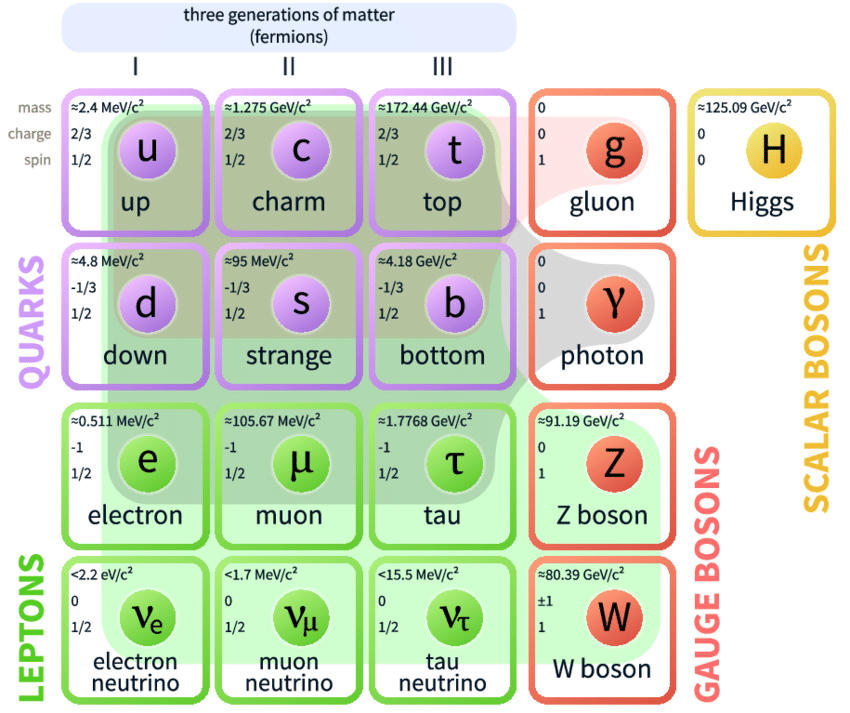
\includegraphics[width=0.75\textwidth]{figures/chapter_SM/SM}
%            \caption{
%                A schematic diagram of the Standard Model Particles seen in the scale of the experiment of the Large Hadron Collider
%                \cite{enwiki:1060203113}.
%            }
%            \label{fig:SM}
%        \end{center}
%    \end{figure}
%

%\section{Experimental Measurement}
%\label{sec:ExpMeasurement}
%
%
%%Summary plots 
%
%    \begin{figure}[!htb]
%        \begin{center}
%            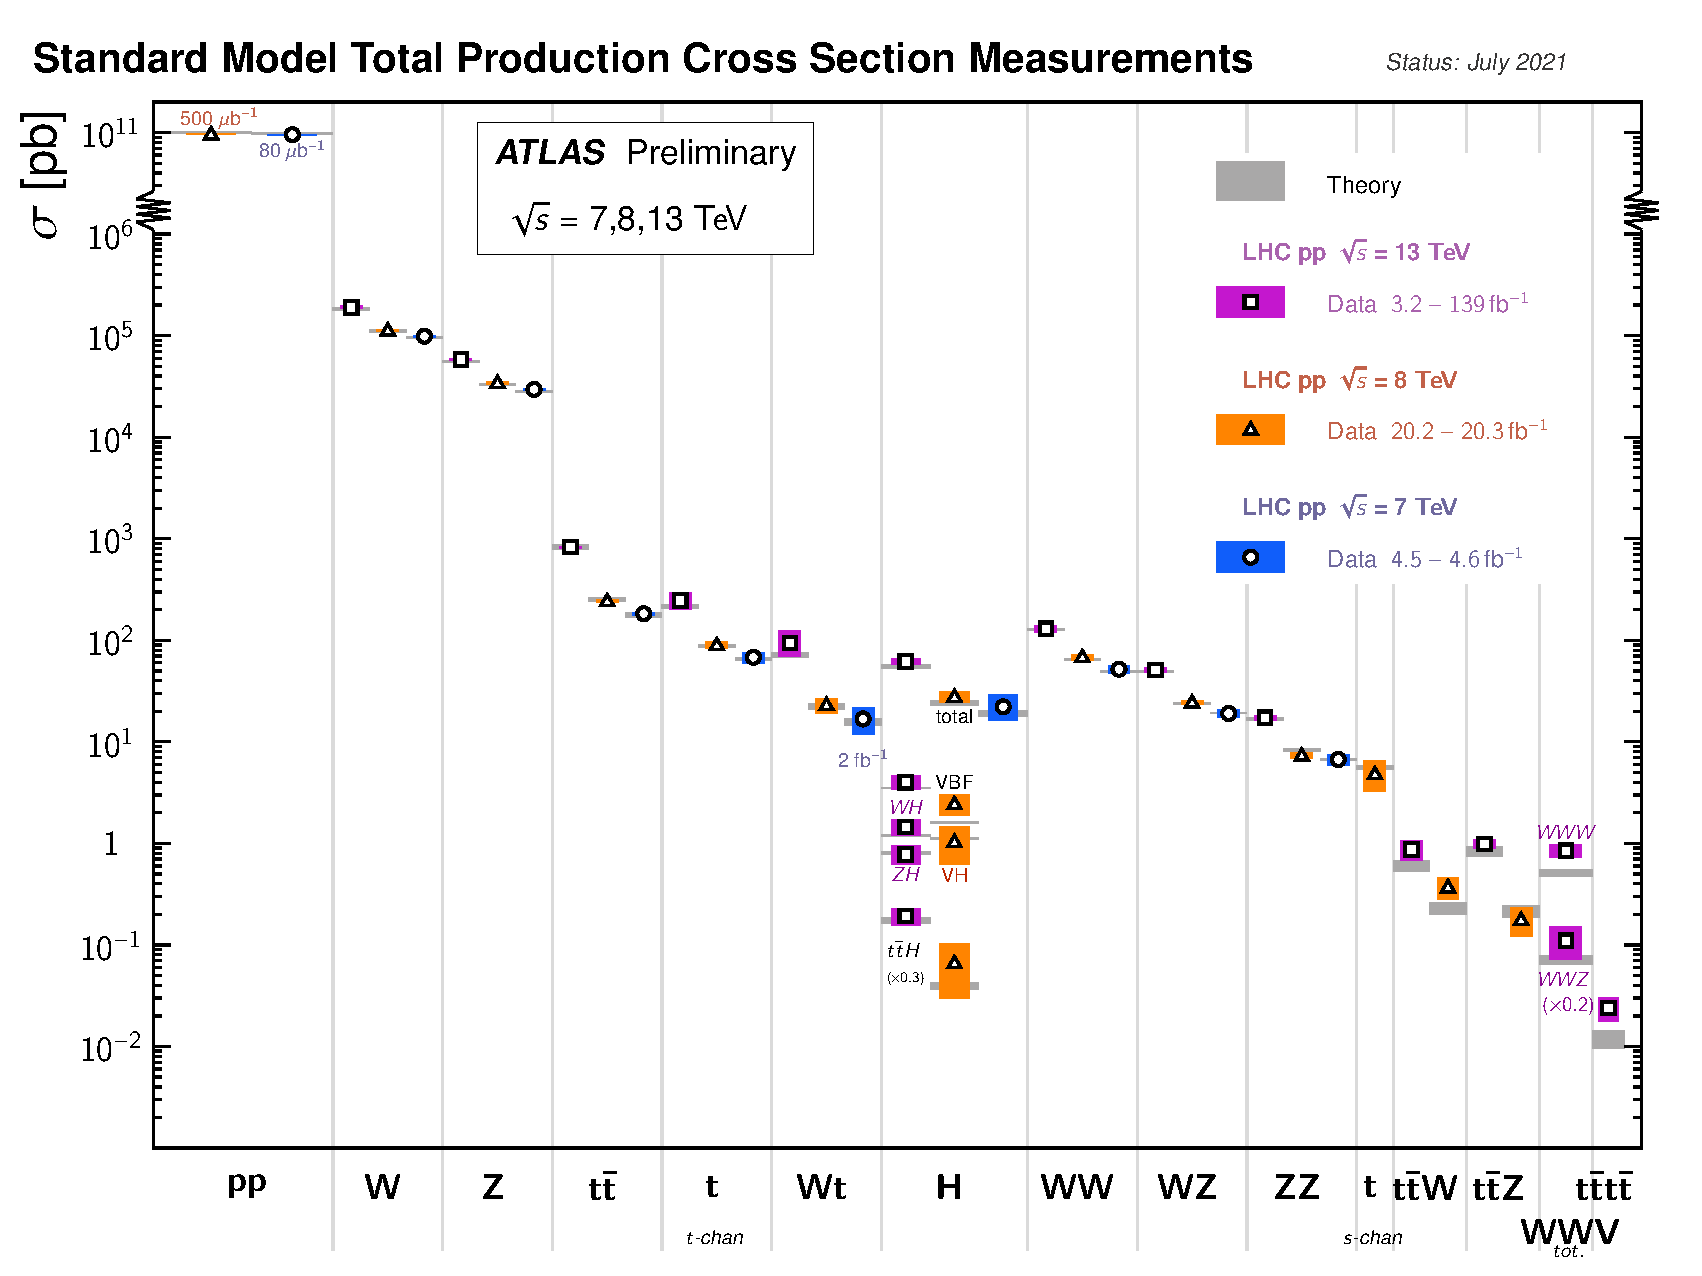
\includegraphics[width=0.75\textwidth]{figures/chapter_SM/SM_Measurement}
%            \caption{
%                A summary plot on the Standard Model cross-section measurements done by the ATLAS experiment~\cite{ATL-PHYS-PUB-2021-032}.
%            }
%            \label{fig:SM}
%
%        \end{center}
%    \end{figure}
%

%\section{Sucessful Prediction}
%\label{sec:ExpConsistency}
%The Standard Model has many successes in the particle level, and it has made along with many successful predictions, these predictions include:
%    \begin{itemize}
%        \item existence of W boson %~\cite{}
%        \item existence of Z boson %~\cite{}
%        \item existence of the charm quark %~\cite{}
%        \item existence of the top quark %~\cite{}
%        \item existence of the Higgs boson %~\cite{}
%    \end{itemize}



\section{Unresolved Problems in the Standard Model}
\label{sec:UnresolvedSM}
The SM in its current forms has had many standing unresolved problems, leading to a consensus in the physics community to believe that a more complete theory is out there to be discovered. These proposed solutions to the SM are called Beyond-the-Standard-Model(BSM) theories. The unresolved problems and testing of the BSM solutions are main motivators to many studies done in the particle physics community. In this section, a list of major known existing problems of the SM are summarized.

\subsection{Gravity}
The Standard Model does not include gravity, one of four fundamental forces. Many attempts to reconcilliating gravity with the existing SM has proved to be challenging\cite{sep-quantum-gravity}.

\subsection{Naturalness}
Naturalness is the property in physics theory where the dimensionless ratio between the free parameters and the physical constants should be in the order of 1. When a physical theory takes either a very large or small value outside the order of 1, they are considered unnatural and unlikely to be "fundamental". 
The Standard Model shows many naturalness issues in different dimensions: 

\subsubsection{The Cosmological Constant Problem}
The Standard Model allows for a 0th dimension constant in its Lagrangian that would not break any of its symmetries. The constant would represent the vacuum energy density and would account for the quantum fluctuation in vacuum. Under Zelokoch's calculations~\cite{zel1968cosmological}, the relations between the vacuum energy density and the cosmological constant of the Einstein's Equation is directly proportional as such:

\begin{equation}
    \rho_{vac}c^2=\Lambda c^4/8\pi G
\label{eq:cosmoconst}
\end{equation}

The cosmological constant is a well-measured value in cosmology from the measurement of the expansion of the universe. The cutting off in either the Planck scale or the electro-weak scale in quantum field theory gives a theoretical prediction value of the vacuum expectation value. However, these values do not match. The experimental measured value of $\rho_{vac}$ is about 40-100 more order of magnitude smaller than the natural theoretical scale. The order of magnitude discrepancy poses the
biggest naturalness issue in the Standard Model~\cite{V2002}.

%Currently, there are proposition that the discrepany could be due to the fact that the neighboring universe is antropologically different than the whole universe[], or modifications could be done to the Einstein's Equation. But as these propositions violates other universal principle or theorems, none are satisfactory.


%In cosmology, it's known that there is a vacuum energy density that exist in the curvature of the universe that can be expressed as the cosmological constant in the Einstein's Equation. The Cosmological constant is measured with the expansion of the universe and would convert to a vacuum 
%In the 0th order, the cosmological constant as measured by experiment is between 40-100 more order of magniture smaller than predicted. 


\subsubsection{The Higgs Hierarchy Problem}
The Higgs hierarchy problem of particle physics describes the apparent large discrepancy in order of magnitude between the electro-weak scale and the gravitational scale, the weak force is about $10^{24}$ greater than gravity. Its effect can be seen in the Higgs mass boson as the mass is 17 order smaller than would be expected by the Planck mass. 
A popular solution is quantum corrections via supersymmetry, but as more phasespace for supersymmetry is being ruled out, this solution is increasingly unlikely to solve the problem and is left to be explored by physicists.

\subsubsection{The Strong CP Problem}
The Standard Model allows for a 4-th dimension term that describes strong CP violation naturally:

\begin{equation}
    \mathcal{L}_{QCD} \supset \theta_{QCD}\epsilon_\mu\nu\rho\sigma \mathcal{G}^{\mu\nu}\mathcal{G}^{\rho\sigma}
\end{equation}

However experimentally, CP violation is not observed: the neutron electro-dipole moment is exceptionally small. Consequentially, the free parameter in the term that describes the CP violation is either exceptionally small or zero. The term's existence in the Lagrangian is therefore "unnatural".
One well-known solution to the strong CP problem is the introduction of the Peccei-Quinn symmetry~\cite{PQSym}, under this solution, the new field will create a term that naturally cancels with the strong CP term. A particle named axion is predicted by this theory. Many experiments has since been on the lookout for the particle, but it's never yet been observed to date.

\subsection{Neutrino Mass}
The Standard Model does not predict neutrino to have a mass, however, this contradicts experimental findings. Neutrino oscillation, the change of neutrino flavor over time or travel distance, is observed in different solar and reactor experiment. Mathematically, this would only be possible if there must be a mixing angle between the neutrino mass eigen states and flavor eigen states of neutrinos. This forces the mass of neutrino to be a non-zero, contradicting the SM.

Minimally, a minor extension to the SM is required for neutrino mass to be possible in the SM. This is known as the $\nv$-SM theory. Currently, there are two leading camps of $\nu$ SM: the former camp treats neutrino as a Dirac field, much like other leptons in the SM; the latter predicts neutrinos as a Majorana field, where the anti-neutrino and the neutrino is the same particle. Further experiments are required to discover the nature of neutrino mass. 

%\subsubsection{Triviality Problem}
%Landau pole + asymmototic freedom 


\subsection{Matter-Antimatter Asymmetry}
While the CKM matrix of SM allow for matter-anti matter asymmetry, the measured value of the parameter in the SM is not large enough to account for its observed value in the universe. However, observationally, a dominating amount of matter over antimatter is necessary to account for the observed universe, which includes the formation of most galactic structure, stars, and planets. BSM physics is necessary to account for the asymmetry. 

\subsection{Flavor Problem}
The mass hierarchy of the quarks and the exceptionally large mass of the top quark are all questions not answered by the SM.

\subsection{Dark Matter}
In experiment, it is estimated that dark matter makes up of 25\% of all matter in the universe, about five times as much as ordinary SM particles. However, they are not accounted for in the SM theoretically.
Neither is Dark energy, which is estimated to take up 70\% of the known content of the universe. Figure~\ref{} shows a pie chart that demonstrates the mass-energy distribution of the universe. More details on the diagram and the proposed solution to dark matter in particle form is covered in chapter~\ref{chapter:DM}.

\section{Summary}
The SM has led to many breakthroughs in the understanding matter in the fundamental level. With the discovery of the Higgs boson in 2008, all the particles predicted by the model are found. Precise measurements are done on all of the eighteen model parameters of the Standard Model are made in different experiments. While there remain many open questions and unanswered issues in the theory, these ruptures to the SM serves as a reminder to a more complete theory out there to be explored.

%As a major motivator to the studies done in this thesis, evidence and hypotheses of dark matter will be examined in length in the next chapter. 

%\section{history}
    %Though the advancement in electrodynamics through the Maxwell's Equations and the progress of Special Relativity, Quantum Theory was re-development with the second quantization\footnote{} , path intergral through the study of Fock, Feynman and Paul Dirac, later led to the development of the quantum field theory.   
    %Paradigm of Quantum field theory, and is the basis where consequent theories in the standard model is based on. 

    %History that lead to the standard model
    %What is the standard model 
%\section{Symmetries}

%1. Electro-Weak theory
%    Q.E.D.
%    Dirac and the problem of annihilation of anti-particle lead to the second quantization, with work from 
%    Gauge theory
%    The unification of eletro-dynamic force and the weak force
%    The Higgs Mechanism / spontaneous symmetry breaking 
%
%4. Quantum Chromodynamics
%    Yang-Mill theory, non-abelian gauge groups. 
%5. Spontaneous Symmetry Breaking 

%-cannot describe atom level in QCD

    %* historically, how it was developed
    %* its sucesses, its predictions lead to W,Z, Higgs boson
    %* Neutrino oscillation or their non-zero mass

%Standard model is the corner stone and a starting point in the journey to particle discoveries, 
